\newcommand{\FishArtSlug}{rock-bass}
\newcommand{\FishName}{Rock Bass}\newcommand{\LatinName}{Ambloplites rupestris}
\newcommand{\BodyDepth}{1.05}\newcommand{\TailFork}{.82}\newcommand{\DorsalStart}{2.30}\newcommand{\DorsalEnd}{4.50}
\newcommand{\Legal}{Open all year; no minimum; rock/yellow/white bass daily bag unlimited on both lake pages.}
\newcommand{\EatingSize}{Thick mid-size fish with enough shoulder for a clean fillet.}
\newcommand{\SizeReason}{No daily limit is not a harvest target; smaller fish cost time and larger adults sustain the population.}
\newcommand{\SkinNote}{stout spines; scale or skin}
\newcommand{\ScaleSkin}{Scale for whole or skin-on cooking, working around the stout dorsal and anal spines. Otherwise leave scales on, fillet, and remove skin flat.}
\newcommand{\FilletMethod}{Cut behind gill plate, follow backbone to tail, then sweep across the broad rib cage. The shoulder carries most usable meat, so keep the first cut tight to the head.}
\newcommand{\RockBassPlate}[2]{%
\begin{center}
\includegraphics[width=\linewidth,height=#2,keepaspectratio]{%
lake-country-fishing/chatgpt/cooking/rock-bass/plates/#1.png}
\end{center}}
\newcommand{\CleaningPlate}{%
\RockBassPlate{cleaning}{2.25in}
\begin{center}\footnotesize
Lift the belly wall; use only the knife tip from vent toward throat.
\end{center}}
\newcommand{\FilletPlate}{%
\RockBassPlate{filleting}{2.25in}
\begin{center}\footnotesize
Start tight behind the operculum; then ride the backbone toward the tail.
\end{center}}
\newcommand{\BoneDiagram}{%
\RockBassPlate{bone-map}{2.65in}
\begin{center}\footnotesize
Flesh side: broad front rib fan and short, firm shoulder-pin row.
\end{center}}
\newcommand{\CookingPlate}{\RockBassPlate{cooking}{2.45in}}
\newcommand{\Debone}{Pull the few firm shoulder pins in their forward angle or remove a narrow V-strip. Recheck the thick shoulder from both directions.}
\newcommand{\TrimNotes}{Remove rib membrane and dark lateral strip. Whole-fish cooks must remove gills, viscera, and kidney line.}
\newcommand{\Prep}{Separate thick shoulders from tails for even timing. A short salt rest firms the flesh; keep refrigerated.}
\newcommand{\CookOne}{Pan-roasted rock bass}\newcommand{\CookOneText}{Brown skin-on or skinless portions, lower heat, and finish gently to \qty{145}{^\circ F}.}
\newcommand{\CookTwo}{Fish cakes}\newcommand{\CookTwoText}{Cook boneless fish to \qty{145}{^\circ F}, cool, flake and inspect again, bind lightly, then brown patties; refrigerate mixture during handling.}
\newcommand{\Advisory}{Wisconsin treats rock bass with panfish for statewide inland advice: under-50 women and children under 15, up to one/week; women 50+ and men, unrestricted. Check lake-specific advice.}
% Telos shared preamble.
%
% Every Telos publication is designed to be printed on a home laser printer,
% one sheet at a time, and carried into a boat or a garage. Two constraints
% follow from that and govern everything below:
%
%   1. Pure monochrome. No value is ever a hue. Emphasis is carried by rule
%      weight, fill, and type, never by color, so a grayscale or black-only
%      printer loses nothing.
%   2. Card density. A "one-pager" is a hard contract: the leaf must fit on a
%      single side of US Letter. The layout is therefore tight by default and
%      the environments below are sized to leave room for a plate.

\documentclass[10pt,letterpaper]{article}

\usepackage[margin=0.55in,includefoot,footskip=0.24in]{geometry}
\usepackage[T1]{fontenc}
\usepackage[utf8]{inputenc}
\usepackage{lmodern}
\usepackage{microtype}
\usepackage{array}
\usepackage{booktabs}
\usepackage{longtable}
\usepackage{tabularx}
\usepackage{enumitem}
\usepackage{needspace}
\usepackage{multicol}
\usepackage{ragged2e}
\usepackage{graphicx}
\usepackage{wrapfig}
\usepackage{xcolor}
\usepackage{fancyhdr}
\usepackage{titlesec}
\usepackage{hyperref}
\usepackage[most]{tcolorbox}
\usepackage{tikz}
\usetikzlibrary{arrows.meta,calc,positioning,shapes.geometric,decorations.pathmorphing,patterns,fadings}

% Semantic names are kept so a document reads intelligibly, but every value is
% black, white, or a neutral gray that survives a black-only print driver.
\definecolor{telosink}{gray}{0}
\definecolor{telospaper}{gray}{1}
\definecolor{telosrule}{gray}{0.35}
\definecolor{telosfill}{gray}{0.90}
\definecolor{telosdeep}{gray}{0.72}
\definecolor{telosmute}{gray}{0.45}

\hypersetup{hidelinks,pdfborder={0 0 0}}

% Keep an unchanged source byte-reproducible across rebuilds: no build-clock
% creation date and no random trailer ID.
\pdfinfoomitdate=1
\pdftrailerid{}

\setlength{\parindent}{0pt}
\setlength{\parskip}{0.42em}
\setlength{\tabcolsep}{4pt}
\setlength{\columnsep}{1.1em}
\renewcommand{\arraystretch}{1.18}
\setlist[itemize]{leftmargin=1.15em,itemsep=0.12em,topsep=0.2em,parsep=0pt}
\setlist[enumerate]{leftmargin=1.5em,itemsep=0.18em,topsep=0.2em,parsep=0pt}
\setlist[description]{leftmargin=0pt,itemsep=0.16em,topsep=0.2em,parsep=0pt,
  font=\normalfont\bfseries}

% ---------------------------------------------------------------------------
% Document identity. Each leaf declares these before \begin{document} so the
% running head, the colophon, and the PDF metadata all agree.
% ---------------------------------------------------------------------------
\newcommand{\TelosProject}{Telos}
\newcommand{\TelosDocTitle}{}
\newcommand{\TelosDocSubtitle}{}
\newcommand{\TelosRevision}{}

\newcommand{\telosmeta}[4]{%
  \renewcommand{\TelosProject}{#1}%
  \renewcommand{\TelosDocTitle}{#2}%
  \renewcommand{\TelosDocSubtitle}{#3}%
  \renewcommand{\TelosRevision}{#4}%
  \hypersetup{pdftitle={#2},pdfsubject={#3; version #4},
    pdfkeywords={Telos, version #4},pdfauthor={Telos}}%
}

\pagestyle{fancy}
\fancyhf{}
\renewcommand{\headrulewidth}{0pt}
\renewcommand{\footrulewidth}{0.4pt}
\fancyfoot[L]{\footnotesize\textsc{\TelosProject}}
\fancyfoot[C]{\footnotesize\TelosDocTitle}
\fancyfoot[R]{\footnotesize\thepage}

% The first page of a one-pager carries the masthead instead of a running foot,
% so its footer is the compact provenance line.
\fancypagestyle{telosfirst}{%
  \fancyhf{}%
  \renewcommand{\headrulewidth}{0pt}%
  \renewcommand{\footrulewidth}{0.4pt}%
  \fancyfoot[L]{\footnotesize\textsc{\TelosProject}}%
  \fancyfoot[C]{\footnotesize\TelosRevision}%
  \fancyfoot[R]{\footnotesize\thepage}%
}

% ---------------------------------------------------------------------------
% Masthead. A heavy rule, the title, a light subtitle, a thin rule. The
% optional argument is a right-aligned tag (a species' scientific name, a
% lesson number) that sits on the title's baseline.
% ---------------------------------------------------------------------------
\newcommand{\telosmasthead}[1][]{%
  \thispagestyle{telosfirst}%
  \begingroup
  \setlength{\parskip}{0pt}%
  \noindent\rule{\linewidth}{1.6pt}\par
  \vspace{0.30em}
  \noindent
  \begin{minipage}[b]{0.66\linewidth}
    \raggedright{\LARGE\bfseries\TelosDocTitle}
  \end{minipage}%
  \hfill
  \begin{minipage}[b]{0.32\linewidth}
    \raggedleft{\small\itshape #1}
  \end{minipage}\par
  \vspace{0.18em}
  \noindent{\small\TelosDocSubtitle}\par
  \vspace{0.28em}
  \noindent\rule{\linewidth}{0.4pt}\par
  \endgroup
  \vspace{0.35em}
}

% ---------------------------------------------------------------------------
% Headings. Compact, small-caps, rule-anchored — a card has no room for the
% article class's default vertical air.
% ---------------------------------------------------------------------------
\titleformat{\section}{\normalfont\large\bfseries}{}{0pt}{}[\vspace{-0.55em}\rule{\linewidth}{0.4pt}]
\titlespacing*{\section}{0pt}{0.85em}{0.35em}
\titleformat{\subsection}{\normalfont\normalsize\bfseries}{}{0pt}{}
\titlespacing*{\subsection}{0pt}{0.6em}{0.2em}
\titleformat{\subsubsection}{\normalfont\small\bfseries\scshape}{}{0pt}{}
\titlespacing*{\subsubsection}{0pt}{0.45em}{0.12em}

% A short run-in heading for card interiors that must not consume a full line.
\newcommand{\telosrubric}[1]{\textbf{#1}\enspace}

% Cross-reference helper. Every Telos project is a set of loose printed sheets,
% so a reference names the sheet rather than a page number.
\newcommand{\sheetref}[1]{\textit{see the \textbf{#1} sheet}}

% Which decision, ADR or sheet governs the paragraph you are reading. A reader
% who disagrees with an instruction should be able to find the reasoning behind
% it rather than having to take it on trust.
\newcommand{\governedby}[1]{{\footnotesize\textsc{governed by #1}}}

% ---------------------------------------------------------------------------
% Quantities. siunitx is not in this TeX Live split, and the guides need only a
% fixed thin space and upright units, so define that directly rather than take
% a package dependency the documented install would not satisfy.
%   \qty{9}{kV}  ->  9 kV        \unitof{kV}  ->  kV
% ---------------------------------------------------------------------------
\newcommand{\unitof}[1]{\ensuremath{\mathrm{#1}}}
\newcommand{\qty}[2]{#1\,\unitof{#2}}
\newcommand{\numrange}[2]{#1\,--\,#2}
\newcommand{\qtyrange}[3]{#1\,--\,#2\,\unitof{#3}}
% Inches and feet appear constantly in the fishing guide; keep one spelling.
\newcommand{\inch}[1]{#1\,in}
\newcommand{\feet}[1]{#1\,ft}

% ---------------------------------------------------------------------------
% Cards and boxes.
% ---------------------------------------------------------------------------

% Titled card with a hairline frame. The default card for facts a reader looks
% up rather than reads through.
\newtcolorbox{teloscard}[1]{
  enhanced, breakable,
  colback=telospaper, colframe=telosink, colbacktitle=telospaper,
  coltitle=telosink,
  boxrule=0.5pt, sharp corners,
  left=6pt, right=6pt, top=4pt, bottom=4pt,
  toptitle=3pt, bottomtitle=3pt, titlerule=0.4pt,
  before skip=6pt, after skip=6pt,
  title={#1}, fonttitle=\small\bfseries
}

% Untitled left-ruled block: hierarchy without a redundant label.
\newtcolorbox{telosframe}{
  enhanced, breakable,
  colback=telospaper, frame hidden, boxrule=0pt, sharp corners,
  borderline west={1.3pt}{0pt}{telosink},
  left=8pt, right=2pt, top=3pt, bottom=3pt,
  before skip=6pt, after skip=6pt
}

% Filled emphasis panel — the "read this first" block. The 10% fill stays
% legible under a cheap laser toner curve and still reads as distinct.
\newtcolorbox{telospanel}[1]{
  enhanced, breakable,
  colback=telosfill, colframe=telosink, colbacktitle=telosfill,
  coltitle=telosink,
  boxrule=0.5pt, sharp corners,
  left=6pt, right=6pt, top=4pt, bottom=4pt,
  toptitle=3pt, bottomtitle=3pt, titlerule=0.4pt,
  before skip=6pt, after skip=6pt,
  title={#1}, fonttitle=\small\bfseries
}

% Hazard block. Deliberately the heaviest object on any page: a 1.4pt frame
% plus a solid title bar. Nothing else in Telos is allowed to look like this,
% so a reader skimming a lesson cannot mistake it for ordinary emphasis.
\newtcolorbox{teloshazard}[1]{
  enhanced, breakable,
  colback=telospaper, colframe=telosink,
  colbacktitle=telosink, coltitle=telospaper,
  boxrule=1.4pt, sharp corners,
  left=6pt, right=6pt, top=5pt, bottom=5pt,
  toptitle=3pt, bottomtitle=3pt,
  before skip=8pt, after skip=8pt,
  title={\MakeUppercase{#1}}, fonttitle=\small\bfseries
}

% A stop-and-check gate. Used before anything destructive, and before anything
% that would be expensive to discover later. Shared by every project that has
% a procedure someone could get hurt following carelessly.
\newtcolorbox{gate}[1]{
  enhanced, breakable,
  colback=telospaper, colframe=telosink,
  boxrule=1.0pt, sharp corners,
  left=6pt, right=6pt, top=4pt, bottom=4pt,
  toptitle=3pt, bottomtitle=3pt, titlerule=0.4pt,
  before skip=7pt, after skip=7pt,
  colbacktitle=telospaper, coltitle=telosink,
  title={\MakeUppercase{#1}}, fonttitle=\small\bfseries
}

% ---------------------------------------------------------------------------
% Rating dots. A five-step scale that prints identically in black-only: filled
% versus open circles, never a shaded bar.
% ---------------------------------------------------------------------------
\newcommand{\telosdot}{\tikz[baseline=-0.42ex]\fill[telosink] (0,0) circle (0.28ex);}
\newcommand{\telosopendot}{\tikz[baseline=-0.42ex]\draw[telosink,line width=0.28pt] (0,0) circle (0.28ex);}
\makeatletter
\newcounter{telos@rate}
\newcommand{\telosrating}[1]{%
  \begingroup
  \setcounter{telos@rate}{0}%
  \@whilenum\value{telos@rate}<#1\do{\telosdot\kern0.22em\stepcounter{telos@rate}}%
  \@whilenum\value{telos@rate}<5\do{\telosopendot\kern0.22em\stepcounter{telos@rate}}%
  \endgroup
}
\makeatother

% ---------------------------------------------------------------------------
% Tables.
%
% tabularx reads its body by scanning for a literal \end{tabularx}, so it can
% never be wrapped in a \newenvironment. Documents therefore open tabularx and
% longtable directly and take their house style from these column types and the
% booktabs rules. The one exception is the fact strip below, which is built on
% plain tabular precisely so it *can* be an environment.
% ---------------------------------------------------------------------------
\newcolumntype{L}{>{\raggedright\arraybackslash}X}
\newcolumntype{R}{>{\raggedleft\arraybackslash}X}
\newcolumntype{C}{>{\centering\arraybackslash}X}
\newcolumntype{B}{>{\bfseries\raggedright\arraybackslash}X}
\newcolumntype{N}{>{\raggedright\arraybackslash}p{0.16\linewidth}}

% Key/value fact strip. Two flush columns of short lookups; the label column is
% a fixed fraction so a stack of cards aligns across the whole guide.
\newenvironment{telosfacts}[1][0.24]
  {\begingroup\small
   \setlength{\parskip}{0pt}%
   \renewcommand{\arraystretch}{1.25}%
   \begin{tabular}{@{}>{\bfseries\raggedright\arraybackslash}p{\dimexpr#1\linewidth\relax}@{\hspace{0.7em}}>{\raggedright\arraybackslash}p{\dimexpr\linewidth-#1\linewidth-0.7em\relax}@{}}}
  {\end{tabular}\par\endgroup}
\newcommand{\telosfact}[2]{#1 & #2\\}

% ---------------------------------------------------------------------------
% Seasonal / diurnal activity bar.
%
% \telosseasonbar{4,3,2,1,1,2,3,3,4,5,4,3} draws a twelve-cell month strip
% where each value 0-5 is a fill height. Height, not gray value, carries the
% signal, so it is exact under any toner curve; the cell is outlined either way
% so an empty month is still visibly a month.
% ---------------------------------------------------------------------------
\newcommand{\telosseasonlabels}{J,F,M,A,M,J,J,A,S,O,N,D}
\newcommand{\telosseasonbar}[1]{%
  \begingroup
  \begin{tikzpicture}[x=1.25em,y=2.1ex,baseline=0pt]
    \foreach \v [count=\i from 0] in {#1} {
      \draw[telosrule,line width=0.3pt] (\i,0) rectangle (\i+0.86,5);
      \ifnum\v>0
        \fill[telosink] (\i,0) rectangle (\i+0.86,\v);
      \fi
    }
    \foreach \m [count=\i from 0] in \telosseasonlabels {
      \node[font=\tiny,anchor=north,inner sep=1.2pt] at (\i+0.43,-0.1) {\m};
    }
  \end{tikzpicture}%
  \endgroup
}

% Four-cell day-part strip: dawn, midday, dusk, night.
\newcommand{\telosdaylabels}{Dawn,Mid,Dusk,Night}
\newcommand{\telosdaybar}[1]{%
  \begingroup
  \begin{tikzpicture}[x=2.9em,y=2.1ex,baseline=0pt]
    \foreach \v [count=\i from 0] in {#1} {
      \draw[telosrule,line width=0.3pt] (\i,0) rectangle (\i+0.92,5);
      \ifnum\v>0
        \fill[telosink] (\i,0) rectangle (\i+0.92,\v);
      \fi
    }
    \foreach \m [count=\i from 0] in \telosdaylabels {
      \node[font=\tiny,anchor=north,inner sep=1.2pt] at (\i+0.46,-0.1) {\m};
    }
  \end{tikzpicture}%
  \endgroup
}

% A bar needs vertical room for its labels when it sits in a fact strip.
\newcommand{\telosbarrow}[1]{\rule{0pt}{4.2ex}#1\rule[-1.6ex]{0pt}{1.6ex}}

% ---------------------------------------------------------------------------
% Plates. A species or apparatus illustration with a caption rule beneath it.
% \telosplate{width fraction}{file}{caption}
% ---------------------------------------------------------------------------
\newcommand{\telosplate}[3]{%
  \begingroup
  \centering
  \includegraphics[width=#1\linewidth]{#2}\par
  \vspace{0.15em}
  \begin{minipage}{#1\linewidth}
    \rule{\linewidth}{0.4pt}\par
    \vspace{0.1em}
    {\footnotesize #3\par}
  \end{minipage}\par
  \endgroup
  \vspace{0.3em}
}

% TikZ drawing conventions shared by every rig, knot, and circuit diagram.
\tikzset{
  telos line/.style={draw=telosink,line width=0.7pt},
  telos hair/.style={draw=telosink,line width=0.35pt},
  telos heavy/.style={draw=telosink,line width=1.2pt},
  telos node/.style={draw=telosink,fill=telospaper,align=center,inner sep=4pt,font=\small},
  telos emphasis/.style={draw=telosink,line width=1.2pt,fill=telospaper,align=center,
    inner sep=4pt,font=\small\bfseries},
  telos label/.style={font=\scriptsize,inner sep=1.5pt},
  telos arrow/.style={-{Stealth[length=1.8mm]},draw=telosink,line width=0.6pt},
  telos dim/.style={|<->|,draw=telosink,line width=0.35pt},
  telos water/.style={draw=telosrule,line width=0.4pt,decorate,
    decoration={snake,amplitude=0.4mm,segment length=3mm}},
}

% ---------------------------------------------------------------------------
% Lesson furniture
% ---------------------------------------------------------------------------

% \lessonhead{number}{time}{who does what}
\newcommand{\lessonhead}[3]{%
  \par\noindent
  \begin{minipage}{\linewidth}
    \rule{\linewidth}{0.4pt}\par
    \vspace{0.3em}
    {\small\textbf{Lesson #1}\quad$\cdot$\quad #2\quad$\cdot$\quad #3\par}
    \vspace{0.25em}
    \rule{\linewidth}{0.4pt}
  \end{minipage}\par
  \vspace{0.5em}}

% The materials list. Two columns of short lines; a lesson that needs a long
% shopping list is a lesson that has not been thought through.
\newenvironment{materials}
  {\begin{telospanel}{What you need}\begin{multicols}{2}
   \begin{itemize}[leftmargin=1em,itemsep=0.05em,topsep=0pt]}
  {\end{itemize}\end{multicols}\end{telospanel}}

% The four rubrics every lesson carries, in the same order every time:
% what you are about to see, what to do, what it means, and what to ask.
\newcommand{\lessonsection}[1]{\section*{#1}\vspace{-0.35em}\rule{\linewidth}{0.4pt}\vspace{0.2em}}

% A prediction box. The point of the curriculum is that they commit to an
% answer before the demonstration, not after.
\newtcolorbox{predict}{
  enhanced, breakable,
  colback=telospaper, colframe=telosink,
  boxrule=0.5pt, sharp corners,
  left=6pt, right=6pt, top=4pt, bottom=4pt,
  before skip=6pt, after skip=6pt,
  borderline west={2.2pt}{0pt}{telosink},
  title={\small\bfseries Predict first}, fonttitle=\small\bfseries,
  colbacktitle=telospaper, coltitle=telosink,
  toptitle=3pt, bottomtitle=3pt, titlerule=0.4pt,
}

% ---------------------------------------------------------------------------
% Colophon. Rendered once, at the end of the last page, in the recovered footer
% area so it never creates a page of its own.
% ---------------------------------------------------------------------------
\newif\ifTelosColophonRendered
\newcommand{\TelosColophonExtra}{}
\newcommand{\TelosColophon}{%
  \ifTelosColophonRendered\else
  \global\TelosColophonRenderedtrue
  \par
  \enlargethispage{0.5in}%
  \vspace{0.3em}%
  \begingroup
  \setlength{\parskip}{0pt}%
  \begin{minipage}{\linewidth}
  \rule{\linewidth}{0.35pt}\par
  \vspace{0.3em}%
  \fontsize{7}{8.2}\selectfont
  \textbf{Telos.} \TelosProject{} — \TelosDocTitle. Revised \TelosRevision.
  \TelosColophonExtra{}
  Project-created text and diagrams are licensed \href{https://creativecommons.org/licenses/by/4.0/}{CC BY 4.0}.
  Incorporated public-domain artwork remains public domain and is credited on
  the plate it appears with. See \texttt{LICENSE} and \texttt{CREDITS.md} in the
  source. Nothing here is professional advice; verify current regulations and
  follow the stated safety procedure.
  \end{minipage}
  \endgroup
  \fi
}
\AtEndDocument{\TelosColophon}

\newcommand{\FishBonePlate}[3]{%
\begin{center}
\begin{tikzpicture}[x=1cm,y=1cm]
\draw[line width=1pt] (0,0) .. controls (1.3,\BodyDepth) and (6.2,\BodyDepth) .. (7.2,0)
 .. controls (6.2,-\BodyDepth) and (1.3,-\BodyDepth) .. (0,0);
\draw[line width=1pt] (0,0)--(-1,.8)--(-\TailFork,0)--(-1,-.8)--cycle;
\draw (2.0,\BodyDepth*.72)--(\DorsalStart,\BodyDepth*1.35)--(\DorsalEnd,\BodyDepth*.73);
\draw (2.3,-\BodyDepth*.72)--(2.9,-\BodyDepth*1.22)--(3.35,-\BodyDepth*.74);
\draw[densely dashed] (1.35,-.77)--(1.35,.77);
\draw[very thick] (1.4,0)--(6.7,0);
\foreach \x in {1.7,2.05,...,4.85}{\draw (\x,0)--(\x-.26,-.68);}
\draw[very thick,dashed] (1.65,.18)--(#1,.18);
\node[font=\scriptsize,anchor=south] at (3.2,.22) {#2};
\node[font=\scriptsize,align=center] at (3.25,-1.25) {rib sweep: shallow blade\\from backbone toward belly};
\node[font=\scriptsize,align=center] at (6.1,.92) {#3};
\end{tikzpicture}
\end{center}}
\newcommand{\YBonePlate}[2]{%
\begin{center}
\begin{tikzpicture}[x=1cm,y=1cm]
\draw[line width=1pt] (0,0) .. controls (1.3,\BodyDepth) and (6.2,\BodyDepth) .. (7.2,0)
 .. controls (6.2,-\BodyDepth) and (1.3,-\BodyDepth) .. (0,0);
\draw[line width=1pt] (0,0)--(-1,.8)--(-\TailFork,0)--(-1,-.8)--cycle;
\draw[very thick] (1.35,0)--(6.7,0);
\foreach \x in {1.75,2.12,...,4.34}{
  \draw (\x,.04)--(\x+.18,.42);
  \draw (\x+.18,.42)--(\x+.02,.68);
  \draw (\x+.18,.42)--(\x+.38,.66);
}
\draw[very thick,densely dashed] (1.52,.78)--(4.85,.78);
\draw[very thick,densely dashed] (1.52,.12)--(4.85,.12);
\draw[very thick,densely dashed] (4.85,-\BodyDepth*.72)--(4.85,\BodyDepth*.72);
\node[font=\scriptsize,anchor=south] at (3.2,.82) {upper cut above fork tips};
\node[font=\scriptsize,anchor=north] at (3.2,.10) {lower cut below Y stems};
\node[font=\scriptsize,align=center] at (5.85,.75) {#1};
\node[font=\scriptsize,align=center] at (3.2,-1.05) {#2};
\end{tikzpicture}
\end{center}}
\telosmeta{Lake Country Fishing · ChatGPT}{Cooking \FishName}{From legal fish to boneless meal}{2026-07-26}
\begin{document}
\telosmasthead[\LatinName\ · kitchen guide]

\begin{teloshazard}{Start with a lawful, cold fish}
Confirm the live Wisconsin DNR rule and consumption advisory for the exact
water, species, length, and date. Kill a retained fish promptly; do not let it
suffocate slowly. Bleed only where lawful and practical, then place it in a
draining ice slurry or on ice. Keep raw fish at or below \qty{40}{^\circ F};
wash hands, knife, and board after contact with viscera.
\end{teloshazard}

\section{Keep or release?}
\begin{tabularx}{\linewidth}{@{}p{.21\linewidth}L@{}}
\toprule
Legal floor & \Legal\\
Preferred table fish & \EatingSize\\
Why & \SizeReason\\
\bottomrule
\end{tabularx}
\textbf{Legal is not the same as desirable.} A fish may be lawful yet a poor
choice because it is a large breeder, exceeds current meal advice, or cannot be
chilled and used promptly.

\section{Dispatch and field care}
\begin{center}

\begin{tikzpicture}[node distance=.5cm, every node/.style={font=\small,align=center}]
\node[draw,minimum width=2.25cm,minimum height=.7cm] (a) {stun firmly\\above brain};
\node[draw,minimum width=2.25cm,minimum height=.7cm,right=of a] (b) {destroy brain\\confirm no reflex};
\node[draw,minimum width=2.25cm,minimum height=.7cm,right=of b] (c) {bleed if chosen\\clean cut at gills};
\node[draw,minimum width=2.25cm,minimum height=.7cm,right=of c] (d) {bag and ice\\drain meltwater};
\draw[-{Latex}] (a)--(b);\draw[-{Latex}] (b)--(c);\draw[-{Latex}] (c)--(d);
\end{tikzpicture}
\end{center}
\begin{enumerate}
\item Use a decisive percussive blow to the skull immediately above and just
behind the eyes. Follow with a spike or narrow knife into the brain cavity.
\item Confirm loss of rhythmic gill movement and eye reflex. If either remains,
repeat immediately. Cut the gill arches only after insensibility.
\item Keep the fish shaded, clean, and cold. Do not soak flesh in warm lake
water. At home, work in small batches and return finished portions to ice.
\end{enumerate}

\newpage
\section{Clean without contaminating the flesh}
\begin{center}
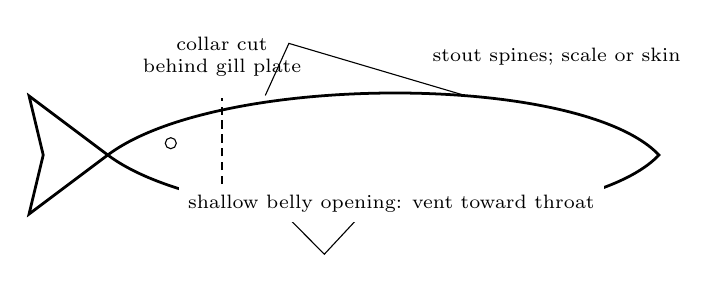
\begin{tikzpicture}[x=1cm,y=1cm]
\draw[line width=1pt] (0,0) .. controls (1.4,\BodyDepth) and (6,\BodyDepth) .. (7,0)
 .. controls (6,-\BodyDepth) and (1.4,-\BodyDepth) .. (0,0);
\draw[line width=1pt] (0,0)--(-1,.75)--(-\TailFork,0)--(-1,-.75)--cycle;
\draw (2.0,\BodyDepth*.72)--(\DorsalStart,\BodyDepth*1.35)--(\DorsalEnd,\BodyDepth*.73);
\draw (2.25,-\BodyDepth*.72)--(2.75,-\BodyDepth*1.20)--(3.2,-\BodyDepth*.74);
\draw (.8,.15) circle (.07);
\draw[densely dashed] (1.45,-.72)--(1.45,.72);
\draw[very thick,-{Latex}] (1.25,-.62)--(5.95,-.62);
\node[font=\scriptsize,fill=white] at (3.6,-.62) {shallow belly opening: vent toward throat};
\node[font=\scriptsize,align=center] at (1.45,1.25) {collar cut\\behind gill plate};
\node[font=\scriptsize,align=center] at (5.7,1.25) {\SkinNote};
\end{tikzpicture}
\end{center}
\begin{enumerate}
\item \textbf{Set up.} Flexible sharp fillet knife, cut-resistant glove on the
non-knife hand, scaler or spoon if needed, pliers, clean towels, two trays.
\item \textbf{Scale or skin.} \ScaleSkin
\item \textbf{Open shallowly.} From vent toward the throat, lift the belly wall
away from organs and use the tip only. Remove viscera intact. Avoid puncturing
the gall bladder; trim and rinse any contaminated tissue.
\item \textbf{Kidney line.} Scrape the dark tissue along the backbone and rinse
briefly with clean potable water. Pat dry. Never use soap on food.
\end{enumerate}

\begin{telospanel}{Parasites and raw fish}
Freezing and pickling are not substitutes for a validated parasite-control
process. Cook wild freshwater fish to an internal temperature of
\qty{145}{^\circ F}, or until opaque and separating easily, unless following a
qualified food-safety process. Discard abnormal-smelling or badly diseased
flesh; when uncertain, do not eat it.
\end{telospanel}

\section{Species-specific first cuts}
\FilletMethod

\newpage
\section{Bone map and deboning}
\BoneDiagram

\begin{enumerate}
\item Keep the skin side down so the blade can ride on, not through, the bones.
\item Remove the rib cage with a shallow sweep, sacrificing as little belly
meat as possible. Run fingertips both directions along every cut surface.
\item \Debone
\item Portion only after a final fingertip inspection under a bright light.
Bones become harder to locate once batter, crumbs, or sauce is added.
\end{enumerate}

\begin{teloscard}{Trim map}
\TrimNotes
\end{teloscard}

\section{Prepare before heat}
\begin{itemize}
\item Pat portions dry. Equal thickness matters more than equal weight.
\item \Prep
\item Refrigerate while the pan, oven, or grill heats. Marinate under
refrigeration; discard marinade that contacted raw fish unless boiled.
\end{itemize}

\newpage
\section{Two dependable methods}
\begin{teloscard}{\CookOne}
\CookOneText
\end{teloscard}
\begin{teloscard}{\CookTwo}
\CookTwoText
\end{teloscard}

\section{Current safe-eating advice · checked 2026-07-26}
\Advisory

\begin{center}

\begin{tikzpicture}[x=1cm,y=1cm]
\node[draw,minimum width=2.2cm,minimum height=.75cm] at (0,0) {1 serving};
\node[anchor=west,font=\small] at (1.35,.22) {adult: about the palm of the hand};
\node[anchor=west,font=\small] at (1.35,-.22) {child: about the child's palm};
\draw[|-|] (-1.1,-.55)--(1.1,-.55);
\node[font=\scriptsize] at (0,-.9) {count all fish meals from all sources};
\end{tikzpicture}
\end{center}

\begin{teloshazard}{The query beats the printed sheet}
Wisconsin has a statewide inland baseline and water-specific exceptions.
Before eating, use DNR's Fish Consumption Advisory Query for Pine Lake
(WBIC 779200) or North Lake (WBIC 850800), and match species and length. People
who are pregnant, may become pregnant, are breastfeeding, and children need
the more protective category. When advice changes, follow the current query.
\end{teloshazard}

{\footnotesize\textbf{Sources.} Wisconsin DNR Eating Your Catch and 2026--27
water-specific regulations; Wisconsin DHS Eat Fish Safely; USDA/FoodSafety.gov
Safe Minimum Internal Temperature Chart; University of Minnesota Extension,
Preserving Food at Home: Meat, Fish and Poultry. Cleaning sequence and
monochrome diagrams are original editorial synthesis, checked 2026-07-26.}
\end{document}

